\documentclass[12pt]{article}
\usepackage{amsmath, amssymb, amscd, amsthm, amsfonts}
\usepackage{graphicx}
\usepackage{hyperref}
\usepackage{commath}
\usepackage{subfig}
\usepackage{float}
\usepackage{listings}
\usepackage{setspace}
\usepackage[T1]{fontenc}
\oddsidemargin 0pt
\evensidemargin 0pt
\marginparwidth 40pt
\marginparsep 10pt
\topmargin -20pt
\headsep 10pt
\textheight 8.7in
\textwidth 6.65in
\linespread{2.0}

\title{ECE656 Project -- Yelp Dataset}
\author{Tiankai Jiang}
\date{\today}

\newtheorem{theorem}{Theorem}
\newtheorem{lemma}[theorem]{Lemma}
\newtheorem{conjecture}[theorem]{Conjecture}

\newcommand{\rr}{\mathbb{R}}

\newcommand{\al}{\alpha}
\DeclareMathOperator{\conv}{conv}
\DeclareMathOperator{\aff}{aff}

\makeatletter
\setlength{\@fptop}{0pt}
\makeatother
\bibliographystyle{ieeetr}

\begin{document}

\maketitle
\section{Introduction}\label{section-introduction}
Yelp dataset is a subset of Yelp's review, business and user data. The Yelp dataset used in this project is 2019 version, which contains 6,685,900 reviews, 192,609 businesses and 1,637,138 users from 10 metropolitan areas. Details of this dataset can be found \href{https://www.yelp.com/dataset/documentation/main}{here}.
\section{Data Preprocessing}\label{section-preprocessing}
\subsection{Data Preview}
We can easily check that all user\_ids in tip.json and review.json have records in user.json. But lots of user\_ids in friends are missing. And we can also check that all business\_ids in tips.json, review.json, checkin.json and photo.json are in business.json. And we can verify that the relationship between friends are mutual, that is, if A appears in B's friend list, then B will appear in A's friend list.

Also, we get the following information: all ids are 22 characters long; maximum username length is 32; maximum business name length is 64; maximum review length is 5000 and maximum tip length is 500. 

The most complex part is the attributes and categories in business information. There are 1300 different categories and 39 different attributes for business. In those attributes, 32 of them have a single value, e.g. "True", "False", "None". The rest of them contain nested structure, which means their value is again, a dictionary. E.g. attribute "BestNights" refers to a dictionary, with each day in a week as a key and "True", "False" as value. Some attributes and categories have a null value, or the field "attribute"/"category" itself is null.

Furthermore, some fields in business.json contain a leading letter "u", e.g. u"True", which means a unicode string. We should remove letter "u" since "True" and u"True" have the same meaning.
\subsection{Data Cleaning}
Remove all user\_ids that appear only in friends list but not in "user\_id" column from user.json. And remove all character "u" before texts from business.json.
\section{Relational Database}\label{section-database}
\subsection{Design}
The ER Diagram of the database is shown as follows. The primary key of a table is in bold and the foreign keys are highlighted in light blue.
% \begin{figure}[H]
% \begin{center}
%     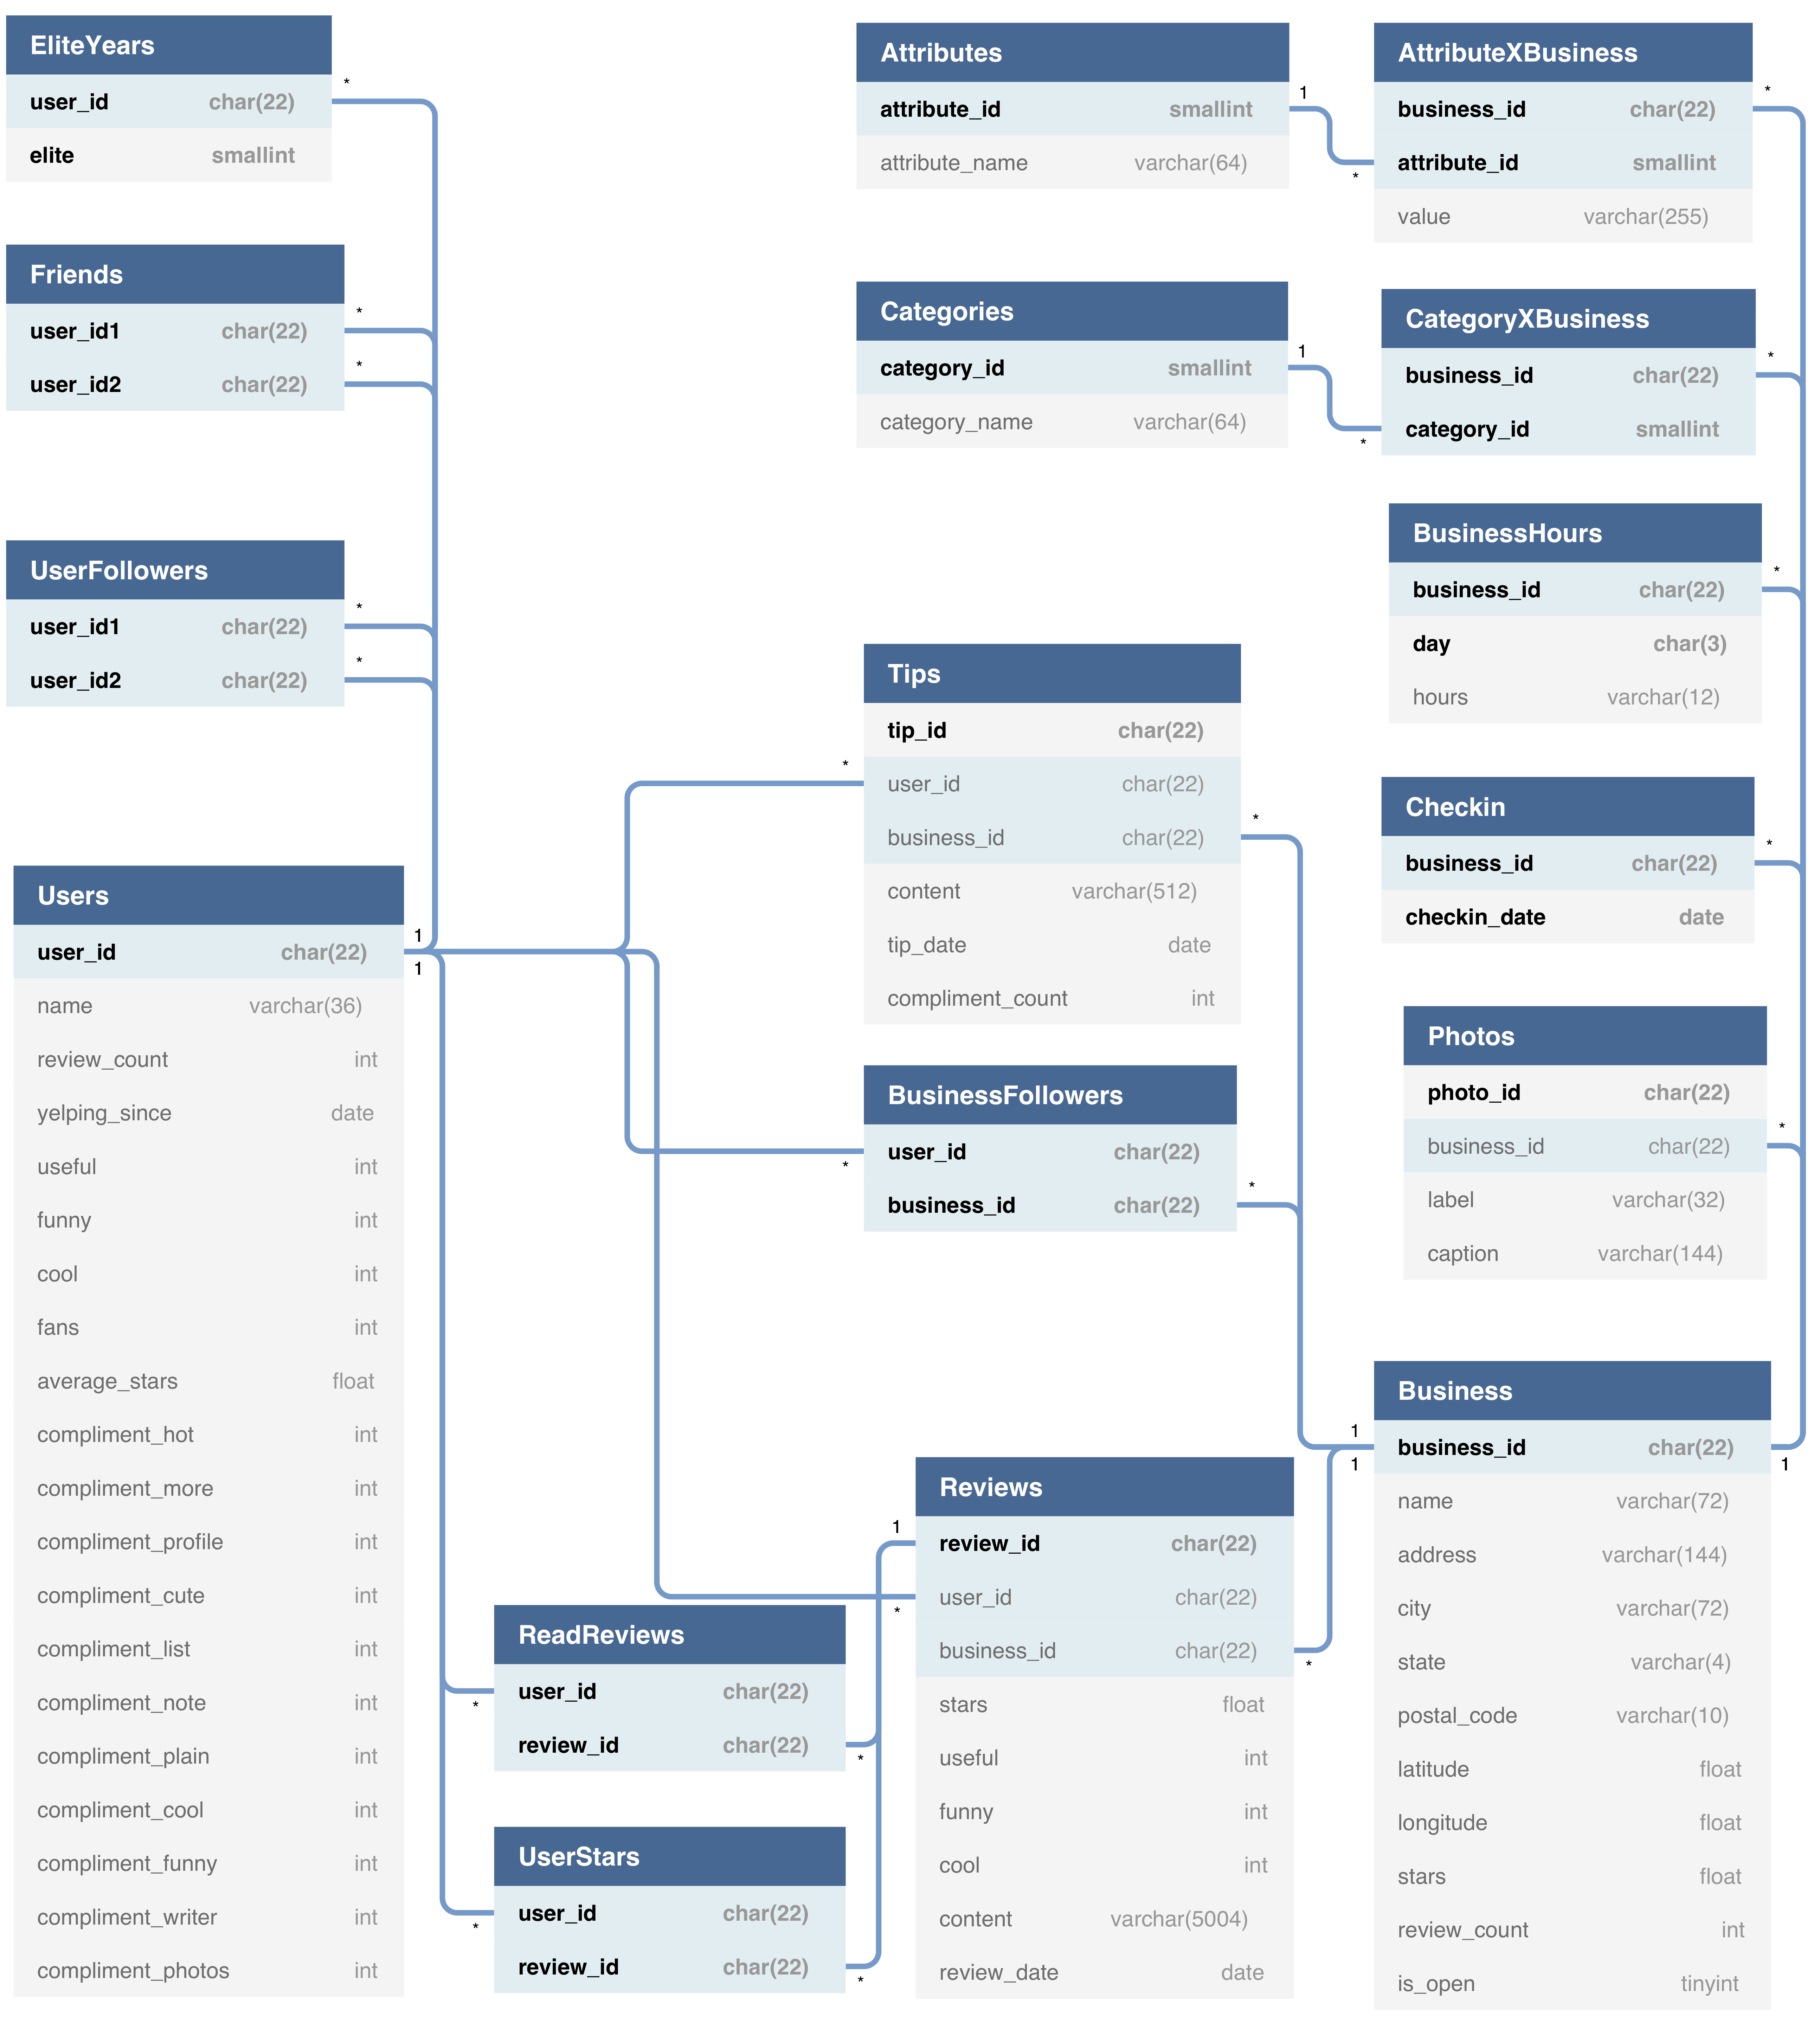
\includegraphics[width=1.0\textwidth]{ER_Diagram.png}
% \end{center}
% \end{figure}
Five main tables in the diagram are {\it Users}, {\it Business}, {\it Reviews}, {\it Photos} and {\it Tips}. Each row of table {\it EliteYears} stores a user\_id and a year number. Table {\it Friends} stores pairs of users. Table {\it Attributes} and table {\it Categories} store ids and names of attributes/categories and connect with {\it Business} through junction table {\it AttributeXBusiness} and {\it CategoryXBusiness}. All values of attributes are stored as string no matter the value is "True"/"False" or a dictionary since they are not our focus in the following analysis, and spliting all of them apart will complicate the design. Table {\it BusinessHours} stores the hours of a business, each day per row, and days are expressed in three characters, from "Mon" to "Sun". Table {\it UserFollowers, BusinessFollowers, ReadReviews} and {\it UserStars} are used for the api and they are not part of the original data.
\subsection{Dumping Data}
Extract all data for tables from json files into individual files, at the same time adding required missing fields such as tip\_id, and then write those files to database. Files should be read as raw string since there are lots of special characters in them.
\section{Server and Client}\label{section-api}
Flask is used as the web framework.
\subsection{API}
8 operations are supported in the API. The status in the responsed json will be 0 if the operation succeeded, otherwise 1, with the error message in message field.

\subsubsection{Login}
\textbf{Description:}\\
Login as an existing user.\\
\textbf{API call:}\\ 
http://127.0.0.1:5000/yelp/login?u=\{user\_id\}\\
\textbf{Parameters:}\\
user\_id: your user\_id\\
\textbf{API Response:}

\begin{singlespacing}
\begin{lstlisting}
{
 "message": "___DPmKJsBF2X6ZKgAeGqg",
 "status": 0
}
\end{lstlisting}
\end{singlespacing}

\subsubsection{Register}
\textbf{Description:}\\
Register a new user account.\\
\textbf{API call:}\\
http://127.0.0.1:5000/yelp/newuser?n=\{username\}\\
\textbf{Parameters:}\\
username: username for the new account\\
\textbf{API Response:}

\begin{singlespacing}
\begin{lstlisting}
{
 "message": "qkVPN3ZeXKxD-2y_bewUEk",
 "status": 0
}
\end{lstlisting}
\end{singlespacing}

\subsubsection{Star/Unstar}
\textbf{Description:}\\
Star/Unstar a review.\\
\textbf{API call:}\\
http://127.0.0.1:5000/yelp/star?u=\{user\_id\}\&r=\{review\_id\}\\
\textbf{Parameters:}\\
user\_id: your user\_id\\
review\_id: an existing review\_id\\
\textbf{API Response:}

\begin{singlespacing}
\begin{lstlisting}
{
 "message": "Starred",
 "status": 0
}
\end{lstlisting}
\end{singlespacing}

\subsubsection{New Review}
\textbf{Description:}\\
Post a new review\\
\textbf{API call:}\\
http://127.0.0.1:5000/yelp/newpost?u=\{user\_id\}\&b=\{business\_id\}\&r=\{content\}\\
\textbf{Parameters:}\\
user\_id: your user\_id\\
business\_id: the business\_id of the business you want to comment on\\
content: review content\\
\textbf{API Response:}

\begin{singlespacing}
\begin{lstlisting}
{
 "message": "NnoOqAoBXsoqOWJVsTakBK",
 "status": 0
}
\end{lstlisting}
\end{singlespacing}

\subsubsection{Follow/Unfollow a User}
\textbf{Description:}\\
Follow/Unfollow a user.\\
\textbf{API call:}\\
http://127.0.0.1:5000/yelp/followu?u=\{user\_id1\}\&f=\{user\_id2\}\\
\textbf{Parameters:}\\
user\_id1: your user\_id\\
user\_id2: user\_id of the person you want to follow\\
\textbf{API Response:}

\begin{singlespacing}
\begin{lstlisting}
{
 "message": "Unfollowed",
 "status": 0
}
\end{lstlisting}
\end{singlespacing}

\subsubsection{Follow/Unfollow a Business}
\textbf{Description:}\\
Follow/Unfollow a business.\\
\textbf{API call:}\\
http://127.0.0.1:5000/yelp/followb?u=\{user\_id\}\&b=\{business\_id\}\\
\textbf{Parameters:}\\
user\_id: your user\_id\\
business\_id: business\_id of the business you want to follow\\
\textbf{API Response:}

\begin{singlespacing}
\begin{lstlisting}
{
 "message": "Followed",
 "status": 0
}
\end{lstlisting}
\end{singlespacing}

\subsubsection{Get All New Reviews1}
\textbf{Description:}\\
Get all new reviews by people you have followed.\\
\textbf{API call:}\\ 
http://127.0.0.1:5000/yelp/ffposts?u=\{user\_id\}\\
\textbf{Parameters:}\\
user\_id: your user\_id\\
\textbf{API Response:}

\begin{singlespacing}
\begin{lstlisting}
{
 "message": [
  {
   "business_id": "Review content1",
   "reviewer": "___DPmKJsBF2X6ZKgAeGqg"
  },
  {
   "business_id": "Review content2",
   "review_id": "GGg4KdkyvbdHwdwsC46l7g",
   "reviewer": "___DPmKJsBF2X6ZKgAeGqg"
  }
 ],
 "status": 0
}
\end{lstlisting}
\end{singlespacing}

\subsubsection{Get All New Reviews2}
\textbf{Description:}\\
Get all new reviews of the business you have followed.\\
\textbf{API call:}\\ 
http://127.0.0.1:5000/yelp/fbposts?u=\{user\_id\}\\
\textbf{Parameters:}\\
user\_id: your user\_id\\
\textbf{API Response:}

\begin{singlespacing}
\begin{lstlisting}
{
 "message": [
  {
   "business_id": "Review content1",
   "reviewer": "___DPmKJsBF2X6ZKgAeGqg"
  },
  {
   "business_id": "Review content2",
   "review_id": "GGg4KdkyvbdHwdwsC46l7g",
   "reviewer": "___QCazm0YrHLd3uNUPYMA"
  }
 ],
 "status": 0
}
\end{lstlisting}
\end{singlespacing}

\subsection{Client}
A simple client to test the api.

\section{Data Mining}\label{section-datamining}
\subsection{Data Visualization}

\end{document}